Dans un système ayant un seul PONE et un seul TARE (en plus du revendeur, du marché de gros et de l'AMI), la demande du client ne peut être satisfaite à cause d'une contrainte que le PONE ne peut satisfaire. Par contre, pendant que le système fonctionne, un PONE est rajouté et il peut fournir l'énergie demandée (en une seule production ou au bout d'un certain nombre de production). L'achat d'énergie devient possible et le reste du déroulement respecte le modèle classique.

Dans notre projet, nous démarrons un PONE 30 secondes aprés le démarrage du lanceur. Ce PONE qui est le PONE pétrole va alors envoyer de l'energie au marché de gros tous comme les autres PONE.
Dans notre projet, pour être sur que celle-ci soit satisfaite dés la 1ère demande (une fois le PONE en marche), nous avons décidé de demander au revendeur du Pétrole mais sans type d'extraction précise avec une quantité de 1.


\begin{figure}[h]
    \centering
    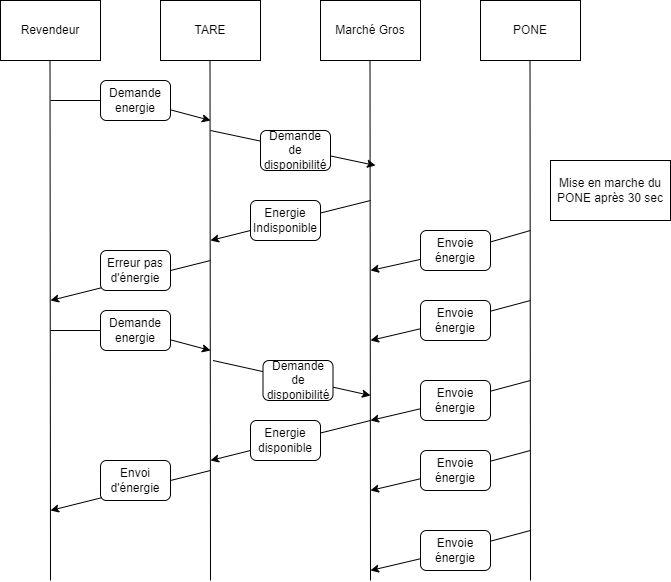
\includegraphics[width=134mm, height=116mm]{images/ScenarioC.png}
    \caption{Schéma du scénario C}
    \label{img:mesh24}
\end{figure}
\newpage